\chapter{Selection and genetic drift}

There are three basic facts about genetic drift that I really want you
to remember, even if you forget everything else I've told you about
it:

\begin{enumerate}

\item Allele frequencies tend to change from one generation to the
next purely as a result of random sampling error. We can specify a
probability distribution for the allele frequency in the next
generation, but we cannot specify the numerical value exactly.

\item There is no systematic bias to the change in allele frequency,
i.e., allele frequencies are as likely to increase from one generation
to the next as to decrease.

\item Populations will eventually fix for one of the alleles that is
initially present unless mutation or migration introduces new
alleles. 

\end{enumerate}

Natural selection introduces a systematic bias in allele frequency
changes. Alleles favored by natural selection {\it tend\/} to increase
in frequency. Notice that word ``tend.'' It's critical. Because there
is a random component to allele frequency change when genetic drift is
involved, we can't say for sure that a selectively favored allele will
increase in frequency. In fact, we can say that there's a chance that
a selectively favored allele {\it won't\/} increase in
frequency. There's also a chance that a selectively {\it dis\/}favored
allele will increase in frequency in spite of natural selection.

\section*{Loss of beneficial alleles}\index{genetic drift!loss of beneficial alleles}

We're going to confine our studies to our usual simple case: one
locus, two alleles. We're also going to consider a very simple form of
directional viability selection in which the heterozygous genotype is
exactly intermediate in fitness.\footnote{Note that if the absolute
  viabilities of $A_1A_1$, $A_1A_2$, and $A_2A_2$ are $w_{11}$,
  $w_{12}$, and $w_{22}$ respectively, then we can write the relative
  fitnesses as $1+s$, $1+hs$, and $1$. We're considering the special
  case where $h=1/2$.}

\begin{center}
\begin{tabular}{ccc}
$A_1A_1$ & $A_1A_2$      & $A_2A_2$ \\
1 + s    & $1 + \half s$ & 1
\end{tabular}
\end{center}

After solving a reasonably complex partial differential equation, it
can be shown that\footnote{Remember, I told you that ``it can be shown
that'' hides a {\it lot\/} of work.} the probability that allele
$A_1$\footnote{The beneficial allele.}  is fixed, given that its
current frequency is $p$ is
\begin{equation}
P_1(p) = \frac{1 - e^{-2N_esp}}{1 - e^{-2N_es}} \quad .
\label{eq:beneficial}
\end{equation}
Now it won't be immediately evident to you, but this equation actually
confirms our intuition that even selectively favored alleles may
sometimes be lost as a result of genetic drift. How does it do that?
Well, it's not too hard to verify that $P_1(p) < 1$.\footnote{Unless
  $p=1$.} The probability that the beneficial allele is fixed is less
than one meaning that the probability it is lost is greater than zero,
i.e., there's some chance it will be lost.

How big is the chance that a favorable allele will be
lost?\index{genetic drift!fixation probability} Well, consider the
case of a newly arisen allele with a beneficial effect. If it's newly
arisen, there is only one copy by definition. In a diploid population
of $N$ individuals that means that the frequency of this allele is
$1/2N$. Plugging this into equation (\ref{eq:beneficial}) above we
find
\begin{eqnarray*}
P_1(p) &=& \frac{1 - e^{-2N_es(1/2N)}}{1 - e^{-2N_es}} \\
       &\approx& 1 - e^{-N_es(1/N)} \hbox{ if $2N_es$ is ``large''} \\
       &=& 1 - e^{s\left(\frac{N_e}{N}\right)} \\
       &\approx& s\left(\frac{N_e}{N}\right)
                 \hbox{ if $s$ is ``small.''}
\end{eqnarray*}
In other words, most beneficial mutations are lost from populations
unless they are {\it very\/} beneficial.\footnote{Notice that it's the
  product of $N_e$ and $s$ that matters, not either one by
  itself. Thus, a population is ``large'' with respect to selection if
  $2N_es > 1$.} If $s=0.2$ in an ideal population, for example, a
beneficial mutation will be lost about 80\% of the time.\footnote{The
  exact calculation from equation (\ref{eq:beneficial}) gives 82\% for
  this probability.} Remember that in a strict harem breeding system
with a single male $N_e \approx 4$ if the number of females with which
the male breeds is large enough. Suppose that there are 99 females in
the population. Then $N_e/N = 0.04$ and the probability that this
beneficial mutation will be fixed is only 0.8\%.

Notice that unlike what we saw with natural selection when we were
ignoring genetic drift, the strength of selection\footnote{i.e., the
  magnitude of differences in relative viabilities} affects the
outcome of the interaction. The stronger selection is the more likely
it is that the favored allele will be fixed. In the case of a newly
arisen allele, it's also {\it only\/} the strength of selection that
matters. Since a newly arisen allele is, by definition exists as only
a single copy, it is very likely to be lost by chance. Once an a
favorable allele has reached an appreciable frequency, the larger the
population is, the more likely the favored allele will be
fixed.\footnote{Because the larger the population, the smaller the
  effect of drift.} Size {\it does\/} matter. But most favorable
alleles are lost before they increase in frequency enough for the
population size to matter.

\section*{Fixation of detrimental alleles}\index{genetic drift!fixation of deleterious alleles}

If drift can lead to the loss of beneficial alleles, it should come as
no surprise that it can also lead to fixation of deleterious ones. In
fact, we can use the same formula we've been using (equation
(\ref{eq:beneficial})) if we simply remember that for an allele to be
deleterious $s$ will be negative. So we end up with
\begin{equation}
P_1(p) = \frac{1 - e^{2N_esp}}{1 - e^{2N_es}} \quad .
\label{eq:deleterious}
\end{equation}
One implication of equation (\ref{eq:deleterious}) that should not be
surprising by now is that even a deleterious allele can become
fixed.\footnote{You might be wondering why I'm not using the same
  approximation here as I did in equation~(\ref{eq:beneficial}), since
  the equations look so similar. The reason is that the exponent on
  $e$ in the denominator is now positive. So $e^{2N_es}$ is the
  biggest term in the denominator instead of the smallest, meaning
  that we can't neglect it.} Consider our two example populations
again, an ideal population of size 100 ($N_e = 100$) and a population
with 1 male and 99 females ($N_e = 4$). Remember, the probability of
fixation for a newly arisen allele allele with no effect on fitness is
$1/2N = 5 \times
10^{-3}$~(Table~\ref{table:fixation}).\footnote{Because
  it's probability of fixation is equal to its current frequency,
  i.e., $1/2N$. We'll return to this observation in a few weeks when
  we talk about the neutral theory of molecular evolution.}

\begin{table}
\begin{center}
\begin{tabular}{l|cc}
\hline\hline
      & \multicolumn{2}{c}{$N_e$} \\
$s$   & 4                  & 100 \\
\hline
0.001 & $4.9 \times 10^{-3}$ & $4.5 \times 10^{-3}$ \\
0.01  & $4.8 \times 10^{-3}$ & $1.5 \times 10^{-3}$ \\
0.1   & $3.2 \times 10^{-3}$ & $2.2 \times 10^{-10}$ \\
\hline
\end{tabular}
\end{center}
\caption{Fixation probabilities for a deleterious mutation as a
function of effective population size and selection coefficient for a
newly arisen mutant ($p=0.01$).}\label{table:fixation}
\end{table}

\section*{Genetic drift and heterozygote advantage}\index{genetic drift!heterozygote advantage}

\begin{itemize}

\item Genetic drift leads to the loss of genetic diversity over time. 

\item Heterozygote advantage leads to the preservation of genetic diversity.

\end{itemize}

You might think that those facts would lead to the conclusion that
drift would cause there to be less diversity than expected as a result
of selection, but that selection would maintain diversity. It would be
nice if the world were that simple. Unfortunately, it's not. 

The key to understanding why is to remember this basic fact: In a
finite population there is a chance that in any generation one of the
alleles that is segregating will be lost. In the absence of mutation
or migration that introduces new genetic diversity into a finite
population, that allele is lost forever. The end result is that {\it
  any\/} finite population will eventually lose its genetic diversity
in the absence of mutation or migration, even one in which selection
is ``trying'' to maintain diversity. Once you realize that, then you
realize that the question isn't ``Will heterozygote advantage maintain
genetic diversity in spite of genetic drift?'' but ``Will heterozygote
advantage retard the inevitable loss of genetic diversity due to
genetic drift?'' The answer to that second questions is ``It depends.''

Specifically, Robertson~\cite{Robertson-1962} showed that if selection
would lead to an equilibrium allele frequency of between about 0.2 and
0.8, then it will tend to retard the loss of genetic diversity. If,
however, selection would lead to a more extreme allele frequency, it
will tend to increase the rate at which diversity is
loss~(Figure~\ref{fig:drift-heterozygote-advantage}). While that
result seems paradoxical at first, after a bit of reflection, it's
somewhat less surprising.

\begin{itemize}

\item If an allele is relatively rare, drift will tend to dominate the
  dynamics of allele frequency change, even if it's under selection.

\item If selection is ``pushing'' an allele to a relatively extreme
  frequency, it will get to the region where drift dominates the
  dynamics more rapidly than it would under drift alone.

\item So heterozygote advantage in which the two homozygotes have very
  asymmetrical fitnesses is likely to increase the rate at which
  diversity is lost. As a corollary, the allele in the disfavored
  homozygote is the most likely to be lost.

\end{itemize}

\begin{figure}
\begin{center}
\resizebox{!}{6cm}{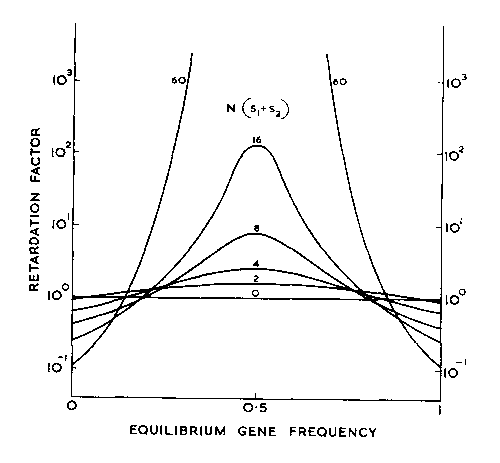
\includegraphics{drift-heterozygote-advantage.eps}}
\end{center}
\caption{The ``retardation factor'' as a function of the equilibrium
  frequency under selection alone and the strength of selection,
  $N(s_1+s_2)$~(from~\cite{Robertson-1962}).}\label{fig:drift-heterozygote-advantage} 
\end{figure}

\section*{Genetic draft}\index{genetic draft}

No. That's not a typo. I meant to type ``genetic draft.'' Genetic
draft is a term that John Gillespie coined~\cite{Gillespie-2000} to
describe a phenomenon similar to genetic drift: If there is ``a steady
stream of adaptive substitutions at one locus$\dots$, [then] the
induced stochastic effects of the substitutions on [a linked] neutral
locus can be faithfully captured in a one-locus model called the {\it
  pseudohitchhiking model}''~\cite[p. 909]{Gillespie-2000} He shows
that the neutral locus shows dynamics that are quite different from
what would be expected if it were not linked to the selective
locus. The effects are illustrated in Figure~\ref{fig:genetic-draft}

\begin{figure}
\begin{center}
\resizebox{!}{8cm}{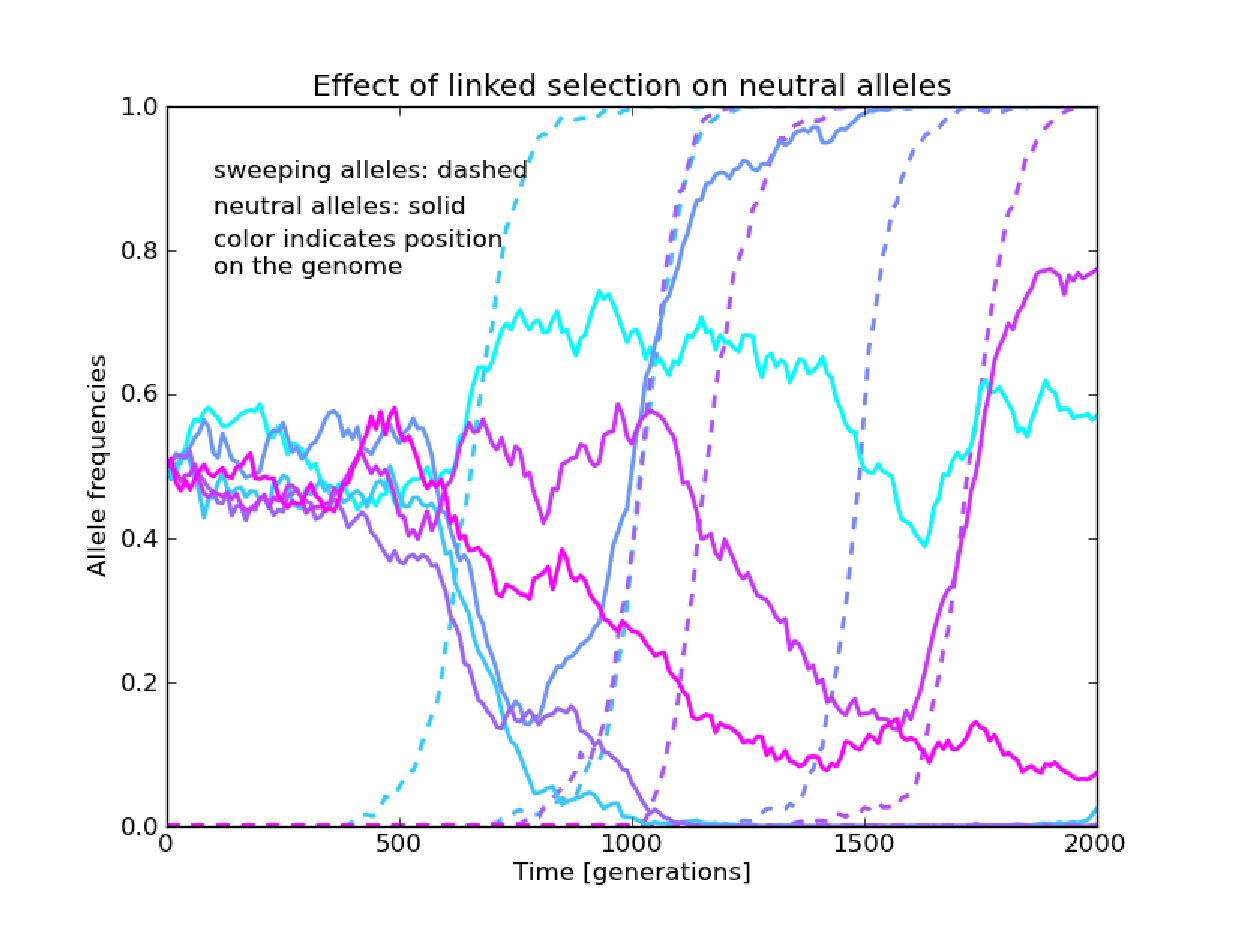
\includegraphics{genetic-draft.eps}}
\end{center}
\caption{The color indicates the position on the genome, selected
  trajectories are in shown as dashed lines, neutral ones by solid
  lines. Neutral allele frequencies are most strongly perturbed by
  sweeps nearby on the chromosome, i.e., of similar color~(from
  {\tt http://webdav.tuebingen.mpg.de/interference/draft.html};
  accessed 27 February 2017).}\label{fig:genetic-draft}  
\end{figure}

\section*{Conclusions}

There are four properties of the interaction of drift and selection
that I think you should take away from this brief
discussion:\index{genetic drift!properties with selection}

\begin{enumerate}

\item Most mutations, whether beneficial, deleterious, or neutral, are
  lost from the population in which they occurred.

\item If selection against a deleterious mutation is weak or $N_e$ is
  small,\footnote{As with mutation and migration, what counts as large
    or small is determined by the product of $N_e$ and $s$. If it's
    bigger than one the population is regarded as large, because
    selective forces predominate. If it's smaller than one, it's
    regarded as small, because drift predominates.} a deleterious
  mutation is almost as likely to be fixed as neutral mutants. They
  are ``effectively neutral.''\index{effectively neutral}\index{genetic drift!effectively neutral}\footnote{We'll
    come back to ``effectively neutral'' when we discuss the neutral
    theory of molecular evolution. It's a very important concept that
    has broader implications than you might guess.}

\item If $N_e$ is large, deleterious mutations are much less likely to
  be fixed than neutral mutations.

\item Even if $N_e$ is large, most favorable mutations are lost.

\item If selection favors heterozygotes, it will retard the loss of
  genetic diversity only when the fitnesses of the two homozygotes are
  not greatly different from one another.

\end{enumerate}

